\documentclass[11pt, a4paper]{article}
\usepackage[margin=1.1in]{geometry}	% edit margins
\usepackage{amsmath}			% for math symbols
\usepackage{graphicx}			% including figures
\usepackage{float}			% placing figures at specific location
\usepackage{amssymb}			% math symbols
\usepackage{soul}			% for highlighting
\usepackage{mathtools}			% for text over equals sign
\newcommand\ivtequal{\stackrel{\mathclap{\normalfont\scriptsize\mbox{FVT}}}{=}}
% \usepackage{./use/mcode}		% for including code


\begin{document}

\title{Final Project: Orbit Determination\\ ASEN 5044 Statistical Estimation}
\author{Keith Covington\\Connor Ott}
\date{December 18, 2019}
\maketitle



%%%%%%%%%%%%%%%%%%%%%%%%%%%%%%%%% INTRODUCTION %%%%%%%%%%%%%%%%%%%%%%%%%%%%%%%%%
\section*{Introduction}
In order to keep track of Earth-orbiting objects, a typical observation scheme includes ground stations which measure range and range-rate to a passing satellite. 
These measurements, when combined with the known locations of the stations, allows for precises estimates of a satellites orbit state. 
In addition to an orbit estimate, it's usually useful to quantify the the uncertainty in the estimate. 
This quantity is a based on the uncertainty in the motion of the satellite in orbit, and the uncertainty in the incoming measurements. 
Neither of these uncertainties are necessarily known.
In order to accurately predict an estimate uncertainty, both of these uncertainties must be balanced with each other. 
This is frequently carried out with predictor-corrector estimation algorithm such as the Linearized Kalman Filter (LKF) or Extended Kalman Filter (EKF.)

In this report, we explore the performance of the LKF and EKF on nonlinear systems with dynamic uncertainty (process noise) and measurement uncertainty (measurement nose.) 
In developing these algorithms, we assume the process and measurement noise are unknown.
We then iterate on different process noise and measurement noise covariance matrices and evaluate the algorithms using \_\_\_\_ (NEES) and \_\_\_\_ (NIS) tests until suitable values for uncertainty are found. 

\section{Part I. Basic System Analysis}

\subsection{CT Model Jacobians}

$\tilde{A}$
$$\left[\begin{matrix}0 & 1 & 0 & 0\\\frac{3\mu x_{1}^{2}}{\left(x_{1}^{2} + x_{3}^{2}\right)^{2.5}} - \frac{\mu}{\left(x_{1}^{2} + x_{3}^{2}\right)^{1.5}} & 0 & \frac{3\mu x_{1} x_{3}}{\left(x_{1}^{2} + x_{3}^{2}\right)^{2.5}} & 0\\0 & 0 & 0 & 1\\\frac{3\mu x_{1} x_{3}}{\left(x_{1}^{2} + x_{3}^{2}\right)^{2.5}} & 0 & \frac{3\mu x_{3}^{2}}{\left(x_{1}^{2} + x_{3}^{2}\right)^{2.5}} - \frac{\mu}{\left(x_{1}^{2} + x_{3}^{2}\right)^{1.5}} & 0\end{matrix}\right]$$

$\tilde{B}$
$$\left[\begin{matrix}0.0 & 0.0\\1.0 & 0.0\\0.0 & 0.0\\0.0 & 1.0\end{matrix}\right]$$

$\tilde{\Gamma}$
$$\left[\begin{matrix}0.0 & 0.0\\1.0 & 0.0\\0.0 & 0.0\\0.0 & 1.0\end{matrix}\right]$$

$\tilde{H}$ - Hmmm
$$\left[\begin{matrix}\frac{x_{1} - x_s}{\left(\left(x_{1} - x_s\right)^{2} + \left(x_{3} - y_s\right)^{2}\right)^{0.5}} & 0 & \frac{x_{3} - y_s}{\left(\left(x_{1} - x_s\right)^{2} + \left(x_{3} - y_s\right)^{2}\right)^{0.5}} & 0\\\frac{\left(- x_{1} + x_s\right) \left(\left(x_{1} - x_s\right) \left(x_{2} - \dot{x}_s\right) + \left(x_{3} - y_s\right) \left(x_{4} - \dot{y}_s\right)\right)}{\left(\left(x_{1} - x_s\right)^{2} + \left(x_{3} - y_s\right)^{2}\right)^{1.5}} + \frac{x_{2} - \dot{x}_s}{\left(\left(x_{1} - x_s\right)^{2} + \left(x_{3} - y_s\right)^{2}\right)^{0.5}} & \frac{x_{1} - x_s}{\left(\left(x_{1} - x_s\right)^{2} + \left(x_{3} - y_s\right)^{2}\right)^{0.5}} & \frac{\left(- x_{3} + y_s\right) \left(\left(x_{1} - x_s\right) \left(x_{2} - \dot{x}_s\right) + \left(x_{3} - y_s\right) \left(x_{4} - \dot{y}_s\right)\right)}{\left(\left(x_{1} - x_s\right)^{2} + \left(x_{3} - y_s\right)^{2}\right)^{1.5}} + \frac{x_{4} - \dot{y}_s}{\left(\left(x_{1} - x_s\right)^{2} + \left(x_{3} - y_s\right)^{2}\right)^{0.5}} & \frac{x_{3} - y_s}{\left(\left(x_{1} - x_s\right)^{2} + \left(x_{3} - y_s\right)^{2}\right)^{0.5}}\\\frac{- x_{3} + y_s}{\left(x_{1} - x_s\right)^{2} + \left(x_{3} - y_s\right)^{2}} & 0 & \frac{x_{1} - x_s}{\left(x_{1} - x_s\right)^{2} + \left(x_{3} - y_s\right)^{2}} & 0\end{matrix}\right]$$ 	


\subsection{DT Linearized Model Matrices}

\subsection{Simulated Nonlinear vs. Linearized System}
Figure \ref{fig:nlvl_s} shows the difference between propagating a small initial perturbation using full nonlinear dynamics and the above DT state transition matrices. 
These were gathered by propagating two orbits, a nominal and initially perturbed orbit, with full nonlinear dynamics using an RK45 integration method.
The difference between these orbits is shown by the blue line in Figure \ref{fig:nlvl_s}. 
The initial perturbation (difference between the initial states of the nonlinear trajectories described above) was then propagated using the linearized DT jacobians evaluated on the nominal trajectory. 
The linear propagation of the perturbation is shown in red. 
The nonlinear and linear perturbations stay near each other for the first half of an orbit, but quickly grow apart.
This indicates that the linearized dynamics are only appropriate for short time spans while the perturbed orbit remains relatively close to the nominal orbit where the DT jacobians are evaluated. 

\begin{figure}[H]
	\centering
	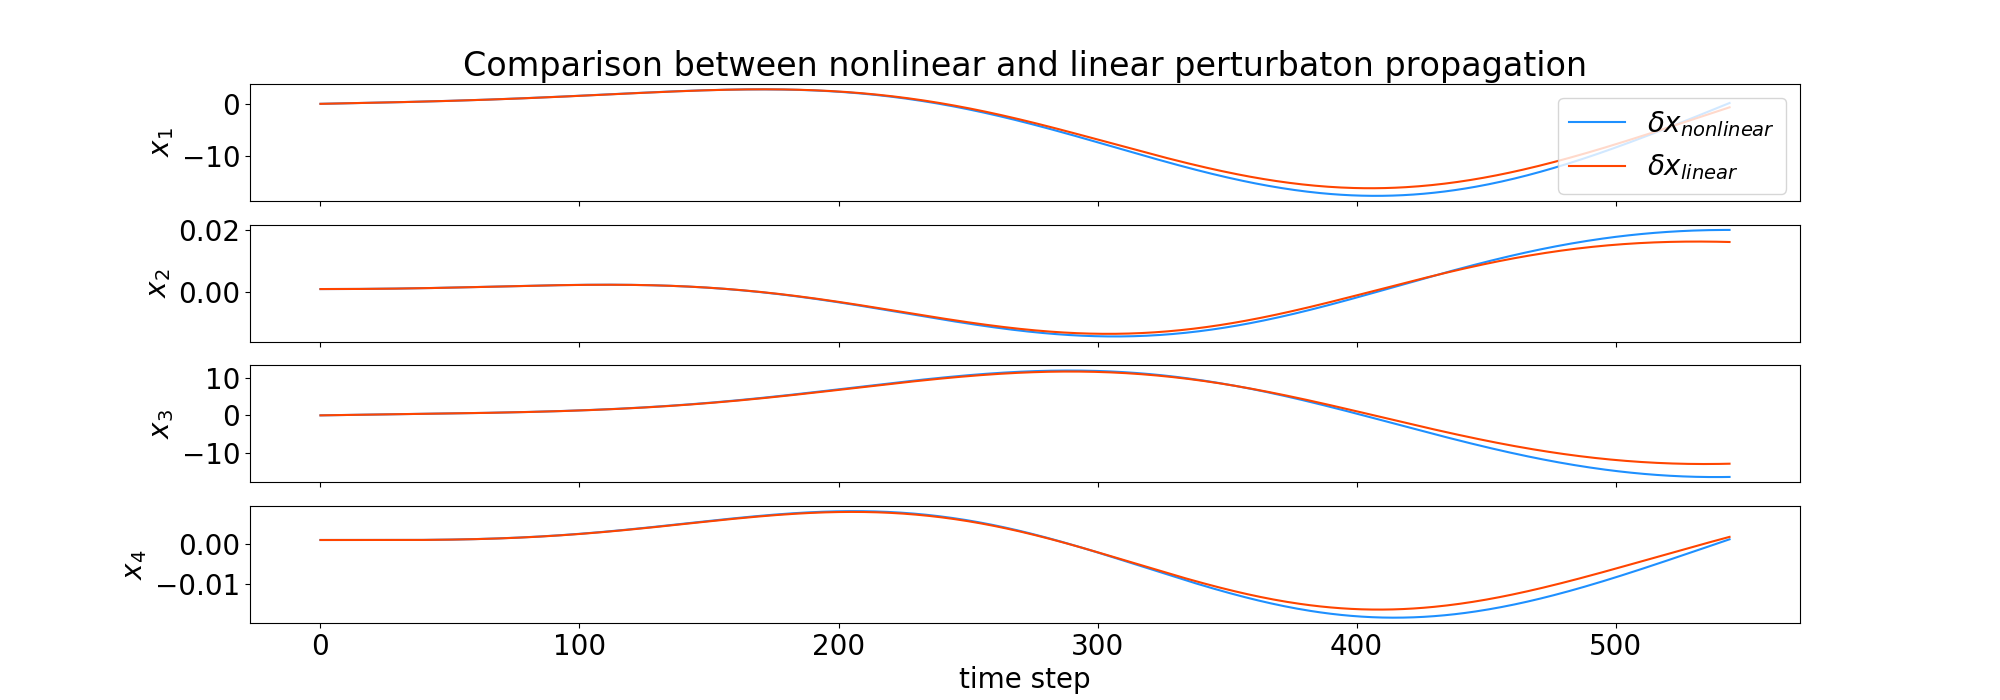
\includegraphics[width=0.8\textwidth]{./Figures/nonlvl_state.png}
	\caption{Comparision between nonlinear and linear perturbation propagation.}
	\label{fig:nlvl_s}
\end{figure}

We draw similar conclusions about the validity of the linearized measurement function from Figure \ref{fig:nlvl_m}.
As the perturbed orbit drifts further and further from the nominal orbit, the linearized dynamics and measurement function are unable to closely match the nonlinear dynamics. 

\begin{figure}[H]
	\centering
	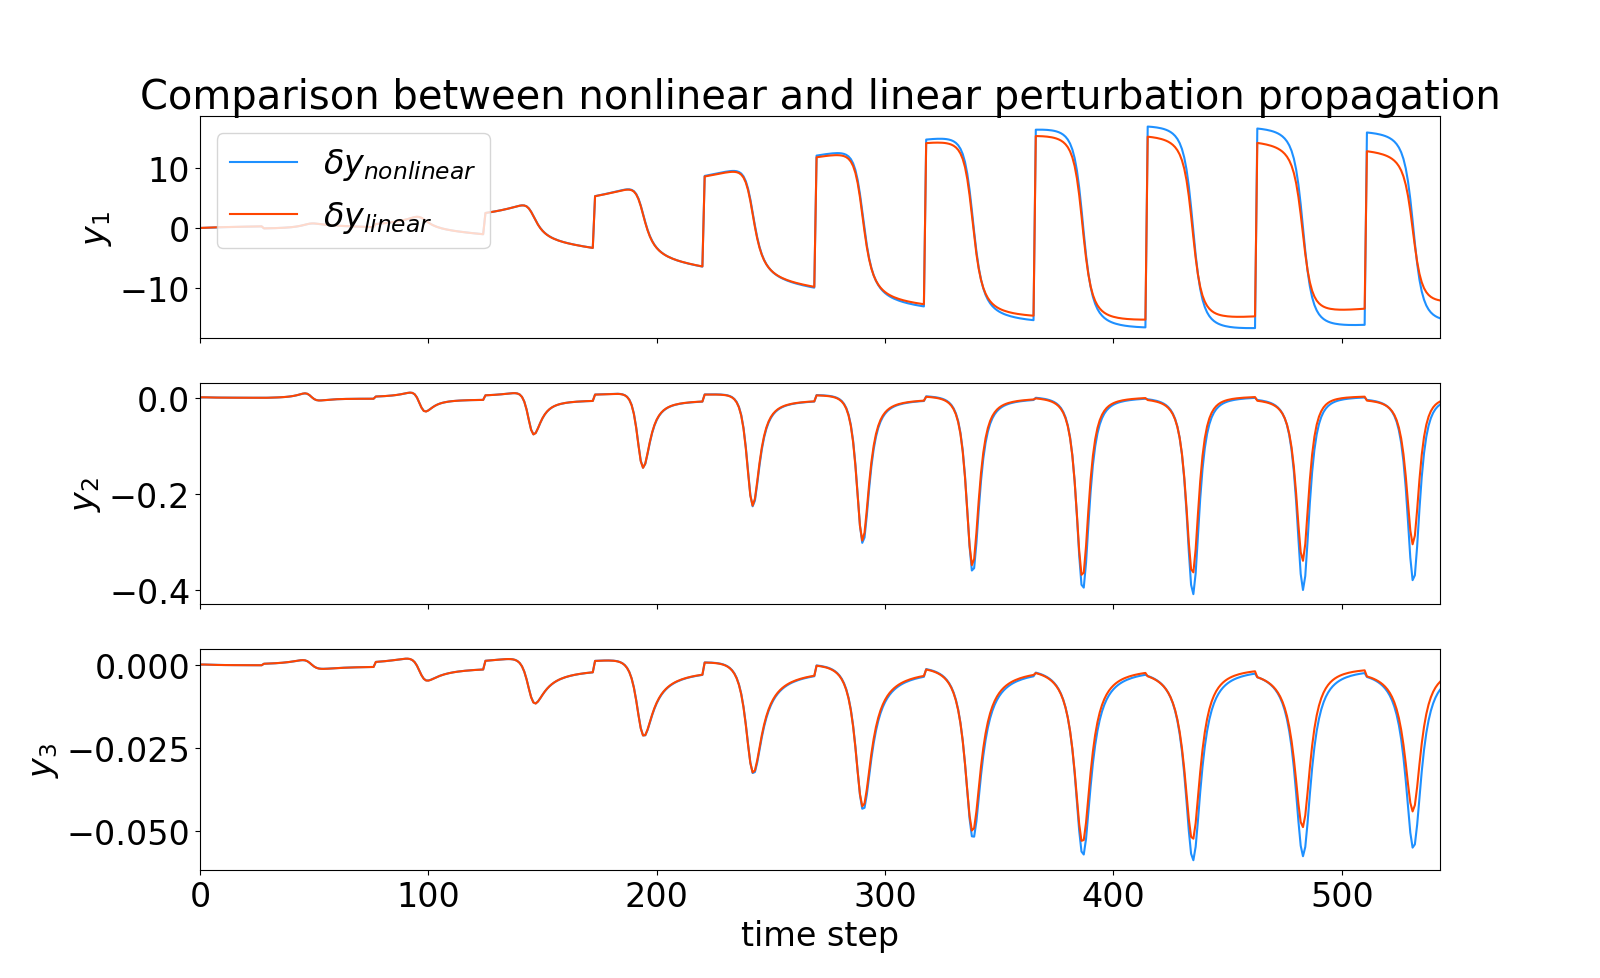
\includegraphics[width=0.8\textwidth]{./Figures/nonlvl_meas.png}
	\caption{Comparision between nonlinear and linear perturbation propagation.}
	\label{fig:nlvl_m}
\end{figure}


\section{Nonlinear Filtering}

\subsection{The Linearized Kalman Filter}
The following are results of NEES and NIS chi-square tests for an implementation of the LKF. \hl{list specs of the sim here when the final figures go in.}

\begin{figure}[H]
	\centering
	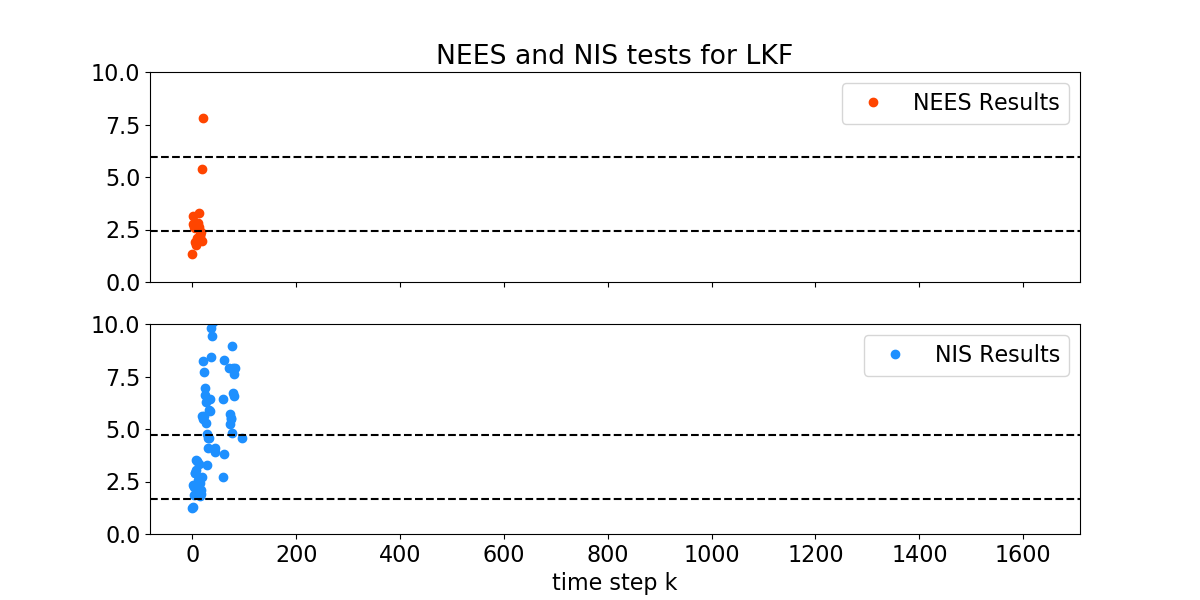
\includegraphics[width=0.8\textwidth]{./Figures/NEESNIS_lkf.png}
	\caption{NEES and NIS chi-square results over time for N= \hl{N} simulated trajectories. Data points continue to grow past ~600 seconds into the analysis.}
	\label{fig:neesnis_lkf}
\end{figure}

The findings in Section I indicated that the linearized dynamics used in the LFK become invalid as small perturbations pull the estimate from the nominal trajectory. 
Figure \ref{fig:neesnis_lkf} corroborates these findings, and solidifies our understanding of where the LKF is most capable, for small perturbations near the nominal trajectory.  





%%%%%%%%%%%%%%%%%%%%%%%%%%%%%%%%% CONCLUSION %%%%%%%%%%%%%%%%%%%%%%%%%%%%%%%%%
\section{Conclusion}




%%%%%%%%%%%%%%%%%%%%%%%%%%%%%%%%% APPENDIX %%%%%%%%%%%%%%%%%%%%%%%%%%%%%%%%%
\newpage
\section*{Appendix}
Attached here is the code used for the numerical analysis and plotting entailed in this project.
%\lstinputlisting{../main.m}


\end{document}


